\documentclass{beamer}

\usepackage{../../../latex_style/beamerthemeExecushares}
\usepackage{../../../latex_style/notations}

\title{Session 6 bis: Markov Chains and PageRank}
\subtitle{Optimization and Computational Linear Algebra for Data Science}
\author{Léo Miolane}
\date{}

\setcounter{showSlideNumbers}{1}

\begin{document}
\setcounter{showProgressBar}{0}
\setcounter{showSlideNumbers}{0}

\frame{\titlepage}

\begin{frame}[t]{Be accurate !}
	\grid

	Let $x,v$ be vectors, $S$ a subspace of $\R^n$ and $M$ an $n \times n$ matrix.

	\vspace{1.5cm}
	\begin{columns}
	\begin{column}{0.45\textwidth}
			\begin{itemize}
				\item $x = S$ or $x \subset S$
	\vspace{0.2cm}
				\item $S \in \R^n$
	\vspace{0.2cm}
				\item $\Span(x,v) = \{a x + b v \}$
	\vspace{0.2cm}
				\item $\dim(M)$ or $\dim(x)$
	\vspace{0.2cm}
				\item $\Ker(M) = 0$
	\vspace{0.2cm}
				\item $x+M$

			\end{itemize}
	\end{column}
	\vrule
	\begin{column}{0.50\textwidth}
	\end{column}
	\end{columns}

\end{frame}


\begin{frame}
	\frametitle{Contents}
	\begin{enumerate}
		\item Markov chains
		\item Perron-Frobenius Theorem
		\item Application: PageRank
		\item A first look at the Spectral theorem.
	\end{enumerate}
\end{frame}


\setcounter{framenumber}{0}
\setcounter{showSlideNumbers}{1}


\section{Markov chains}

\begin{frame}[t]{An example}
	\grid

\end{frame}

\begin{frame}[t]{Stochastic matrices}
	\grid

	\begin{definition}
		A matrix $P \in \R^{n \times n}$ is said to be \emph{stochastic} if:
		\begin{enumerate}
			\item $P_{i,j} \geq 0$ for all $1 \leq i,j \leq n$.
			\item $\sum\limits_{i=1}^n P_{i,j} = 1$, for all $1 \leq j \leq n$.
		\end{enumerate}
	\end{definition}
\end{frame}
\begin{frame}[t]{Probability vectors}
	\grid

\end{frame}

\begin{frame}[t]{The key equation}
	\grid

	\vspace{-0.4cm}
	\begin{block}{Proposition}
		For all $t \geq 0$
		$$
		x^{(t+1)} = P x^{(t)}
		\quad \text{and consequently,} \quad
		x^{(t)} =  P^t x^{(0)}.
		$$
	\end{block}

\end{frame}

\begin{frame}[t]{Long-term behavior}
	\grid


\end{frame}

\section{Perron-Frobenius Theorem}

\begin{frame}[t]{Invariant measure}
	\grid

	\vspace{0.2cm}
	\begin{definition}
		A vector $\mu \in \Delta_n$ is called an invariant measure for the transition matrix $P$ if 
		$$
		\mu = P \mu,
		$$
		i.e.\ if $\mu$ is an eigenvector of $P$ associated with the eigenvalue $1$.
	\end{definition}


\end{frame}

\begin{frame}[t]{Perron-Frobenius Theorem}
	\grid
	\begin{block}{Theorem}
		Let $P$ be a stochastic matrix such that there exists $k \geq 1$ such that all the entries of $P^k$ are strictly positive. Then the following holds:
		\begin{enumerate}
			\vspace{0.3cm}
		\item $1$ is an eigenvalue of $P$ and there exists an eigenvector $\mu \in \Delta_n$ associated to $1$.
			\vspace{0.3cm}
		\item The eigenvalue $1$ has multiplicity $1$: \ $\Ker(P-\Id) = \Span(\mu)$.
			\vspace{0.3cm}
		\item For all $x \in \Delta_n$, $P^t x \xrightarrow[t \to \infty]{} \mu$.
	\end{enumerate}
\end{block}
\end{frame}


\begin{frame}[t]{Consequence}
	\grid
	\begin{block}{Corollary}
		Let $P$ be a stochastic matrix such that there exists $k \geq 1$ such that all the entries of $P^k$ are strictly positive. 
		\\

		Then there exists a unique invariant measure $\mu$ and for all initial condition $x^{(0)} \in \Delta_n$,
		$$
		x^{(t)} = P^t x^{(0)} \xrightarrow[t \to \infty]{} \mu.
		$$
	\end{block}
\end{frame}

\begin{frame}[t]{Proof: Geometrical observations}
	\grid

\end{frame}

\begin{frame}[t]{Proof: contraction}
	\grid

	\vspace{-0.3cm}
	We will prove the theorem in the case where $P_{i,j} > 0$ for all $i,j$.
	\vspace{-0.3cm}
	\begin{lemma}\label{lem:contract}
		The mapping 
		$$
		\begin{array}{cccc}
			\varphi:& \Delta_n &\to& \Delta_n \\
					& x & \mapsto & Px
		\end{array}
		$$
		is a contraction mapping for the $\ell_1$-norm: there exists $c \in (0,1)$ such that for all $x,y \in \Delta_n$:
		$$
		\| Px - Py \|_1 \leq c \| x-y\|_1.
		$$
	\end{lemma}

\end{frame}
\begin{frame}[t]{Geometric picture}
	\grid
\end{frame}
\begin{frame}[t]{Proof of Perron-Frobenius}
	\grid
	\pause
\end{frame}

\section{PageRank}
\begin{frame}[t]{Ordering the Web}
	\grid
\end{frame}

\begin{frame}[t]{Naive attempt}
	\grid

	\textbf{First idea:} rank the webpages according to their number of \emph{incomming links}. (The more incomming links, the more the webpage is important).
\end{frame}

\begin{frame}[t]{The random surfer}
	\grid
\end{frame}

\begin{frame}[t]{PageRank Algorithm}
	\grid

	This defines a Markov chain of transition matrix:
	$$
	P_{i,j} 
	= 
	\begin{cases}
		1 / \deg(j) & \text{if there is a link} \ j \to i \\
		0 & \text{otherwise},
	\end{cases}
	$$

	\vspace{0.6cm}
	\begin{itemize}
		\item After a long time, the surfer is more likely to be on an \emph{important webpage}.
			\vspace{0.3cm}
		\item If $\mu$ is the invariant measure of $P$ (provided $P$ verifies the hypotheses of Perron-Frobenius), we take
			$$
			\mu_i  \ = \ \text{<< importance of webpage}  \ \ i \ \ \text{>>}.
			$$
	\end{itemize}

\end{frame}


\begin{frame}[t]{PageRank Algorithm}
	\grid


\end{frame}

\begin{frame}[t]{Application: ranking Tennis players}
	\grid

	\vspace{0.5cm}
	\textbf{Goal: rank the following players:}
	\begin{center}
		Federer, Nadal, Djokovic, Murray, Del Potro, Roddick, Coria, Zverev, Ferrer, Soderling, Tsonga, Nishikori, Raonic, Nalbandian, Wawrinka, Berdych, Hewitt, Tsitsipas, Monfils, Gonzalez, Thiem, Ljubicic, Davydenko, Cilic, Pouille, Safin, Isner, Dimitrov, Medvedev, Ferrero, Goffin, Bautista Agut, Sock, Gasquet, Simon, Blake, Monaco, Coric, Stepanek, Khachanov, Almagro, Robredo, Verdasco, Anderson, Youzhny, Baghdatis, Dolgopolov, Kohlschreiber, Fognini, Melzer, Paire, Querrey, Tomic, Basilashvili.
	\end{center}
	\vspace{0.5cm}

	\textbf{Data: Head-to Head records} (number of times that player $x$ has defeated player $y$)

\end{frame}

\begin{frame}[t]{Ranking by \% of victories}
	\grid

	\vspace{-1.0cm}
	\begin{center}
		\hspace*{-1.1cm}
		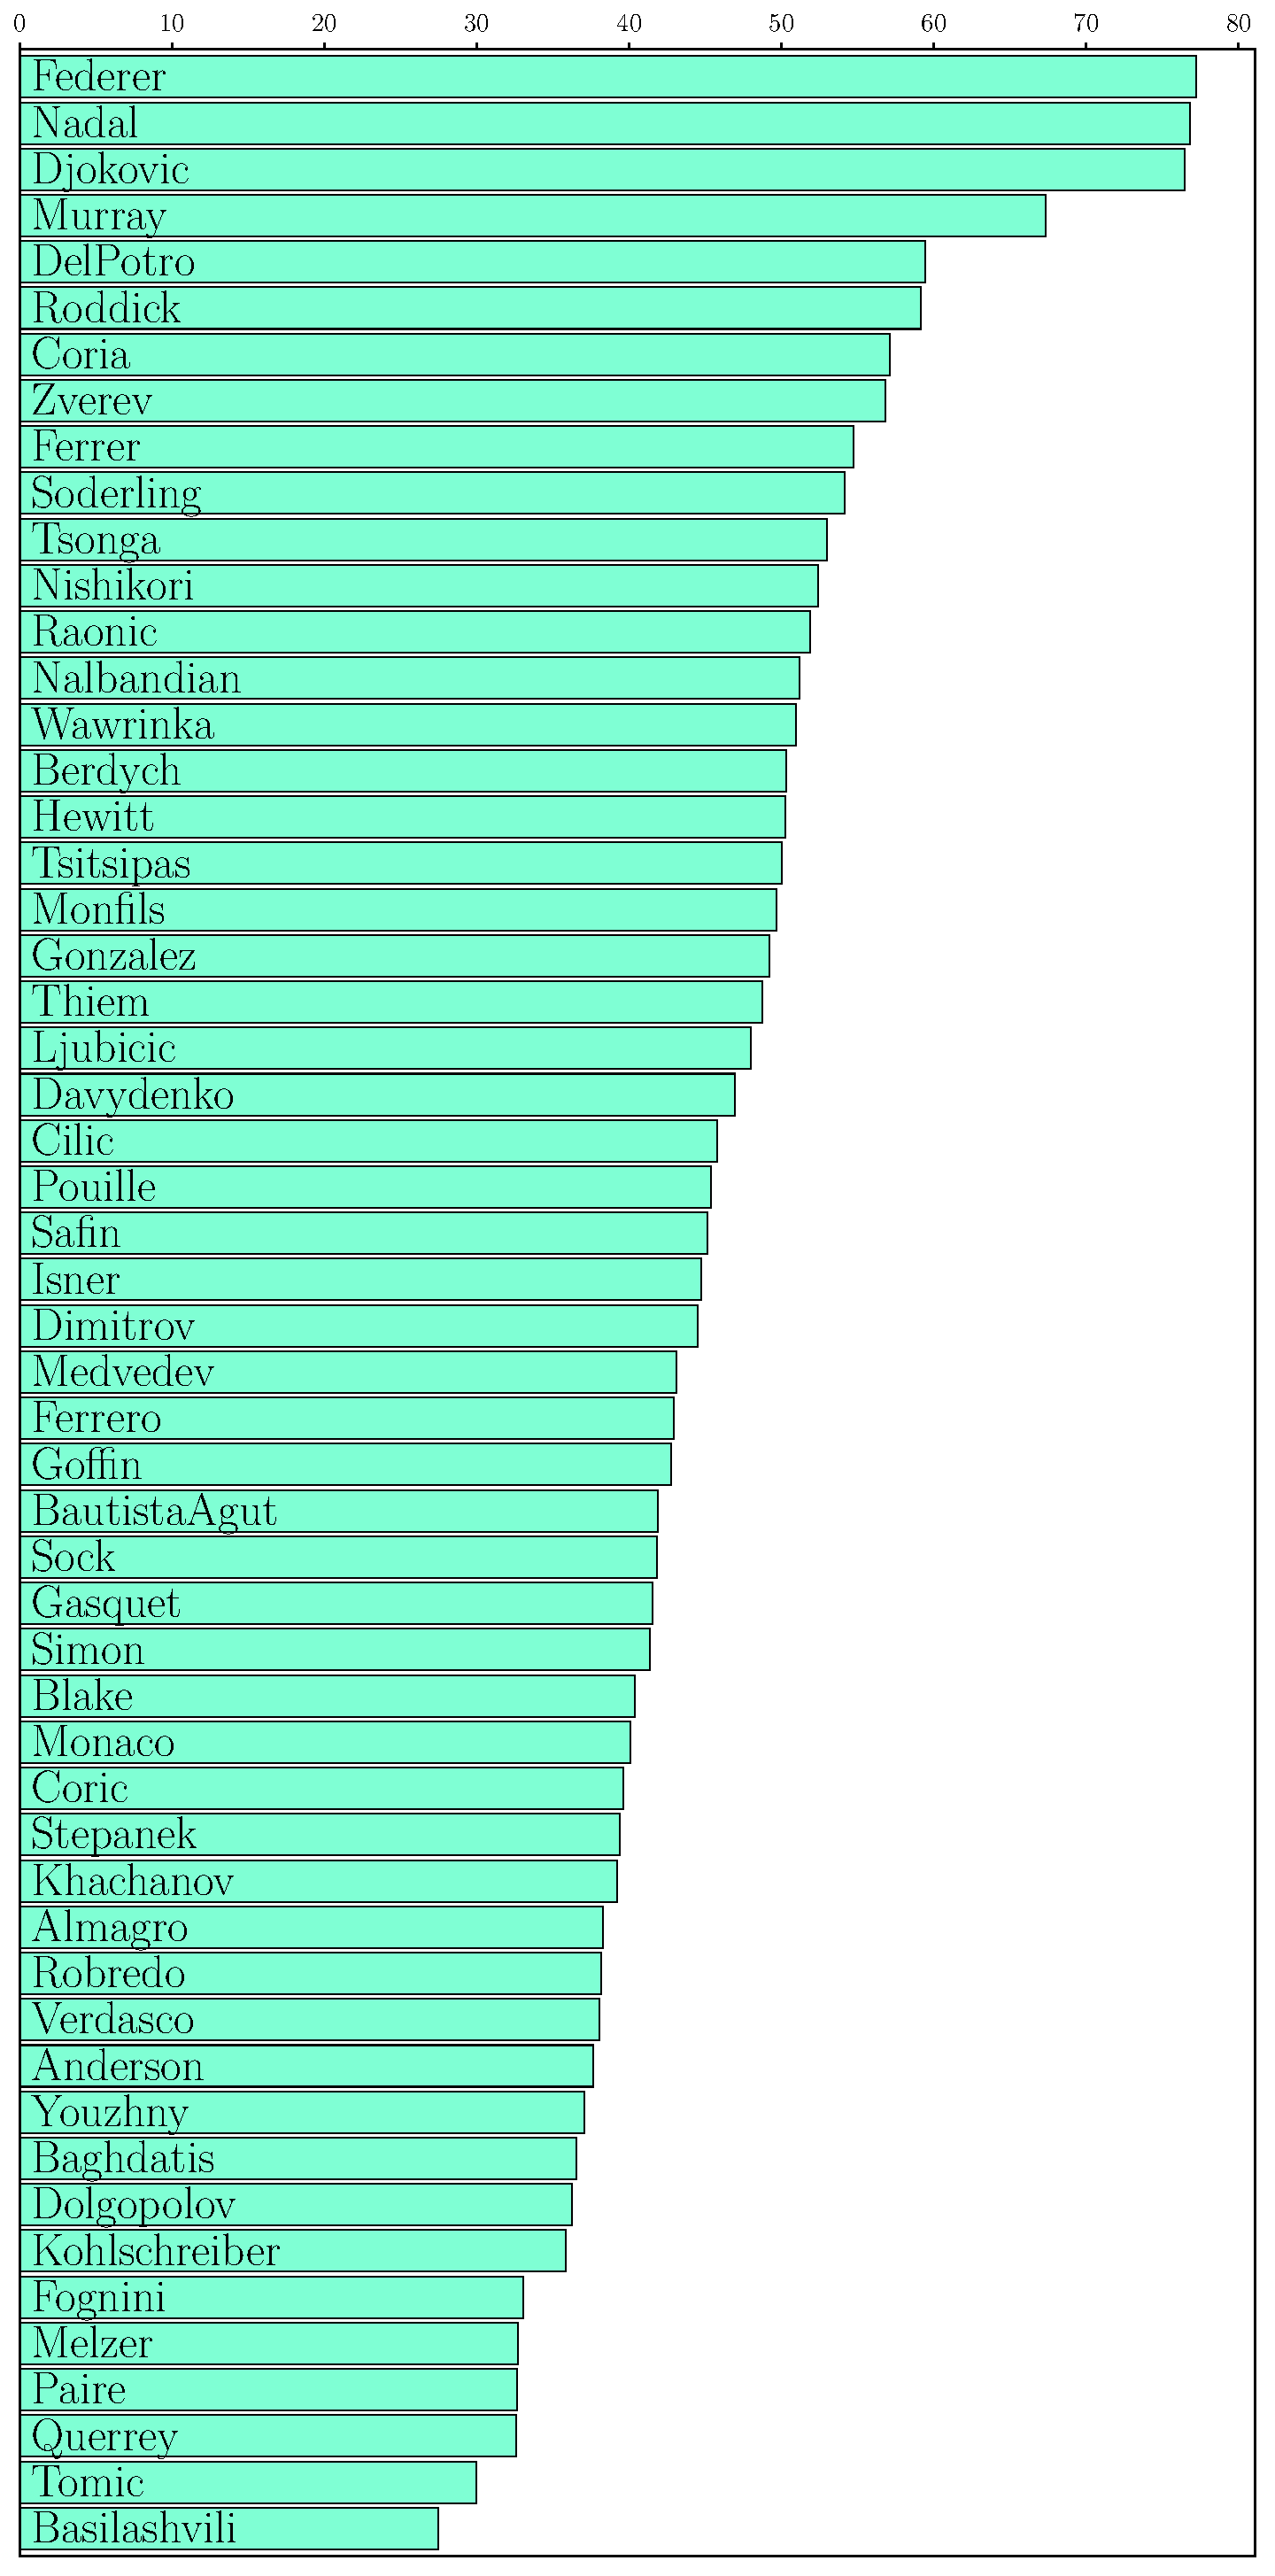
\includegraphics[width=13cm]{../st_tennis.pdf}
	\end{center}
\end{frame}

\begin{frame}[t]{The random spectator}
	\grid

	\vspace{-0.15cm}

	Imagine the following << random spectator >>:

	\vspace{0.15cm}
	\begin{itemize}
		\item At time $t$, the spectator believes that player $j$ is the best: $X_t = j$.
	\vspace{0.3cm}
		\item Then, he picks a game of player $j$ uniformly at random:
	\vspace{0.3cm}

			\begin{itemize}
				\item if player $j$ wins, then the spectator still believes that $j$ is the best: $X_{t+1}=j$.
	\vspace{0.2cm}
				\item otherwise, the spectator changes his mind and now believes that player $i$ who defeated $j$ is the best: $X_{t+1}=i$.
			\end{itemize}
	\end{itemize}

	\pause
	\vspace{0.5cm}
This defines a transition matrix $P$. We rank the players according to the stationary distribution $\mu$ of
$$
M = \alpha P + \frac{1-\alpha}{N} J
$$
\end{frame}

\begin{frame}[t]{Naive ranking vs PageRank}
	\grid

	\vspace{-1.0cm}
	\begin{center}
		\hspace*{-1.3cm}
		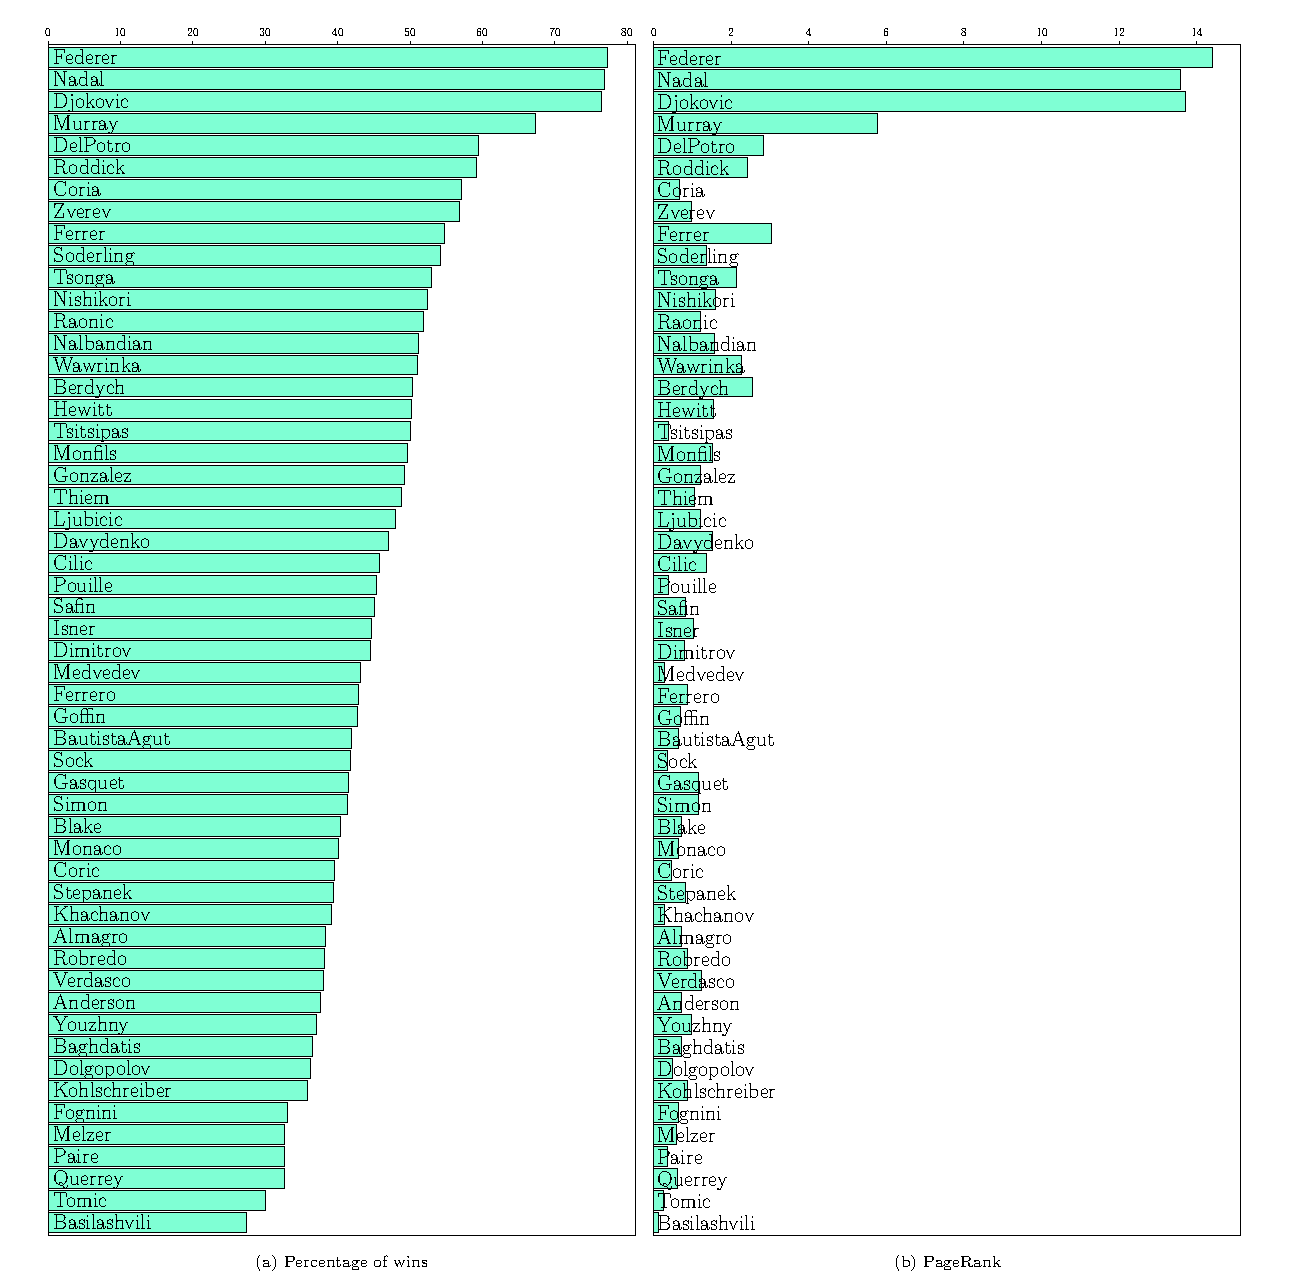
\includegraphics[width=13.5cm]{../pagerank_tennis.pdf}
	\end{center}
\end{frame}

\section{The Spectral Theorem}

\begin{frame}[t]{The spectral theorem}
	\grid
	
	\vspace{-0.3cm}
	\begin{block}{Theorem}
	Let $A \in \R^{n \times n}$ be a \textbf{symmetric} matrix. Then there is a orthonormal basis of $\R^n$ composed of eigenvectors of $A$.
	\end{block}
\end{frame}

\begin{frame}[t]{The spectral theorem}
	\grid
	
\end{frame}

\begin{frame}[t]{Matrix formulation}
	\grid
	
	\vspace{-0.3cm}
	\begin{block}{Theorem}
	Let $A \in \R^{n \times n}$ be a \textbf{symmetric} matrix. Then there exists an orthogonal matrix $P$ and a diagonal matrix $D$ of sizes $n \times n$ such that
	$$
		A = P D P^{\sT}.
	$$
	\end{block}
\end{frame}


\appendix
\backupbegin
\begin{frame}[t]
	\frametitle{Questions?}
	\grid

	\pause
\end{frame}
\backupend

\end{document}
